\section{Hardwarearkitektur}
Dette afsnit beskriver arkitektur for hardware i AutoGreen.

Forsyning til alle blokke er beskrevet på IBD for system, Figur \ref{fig:ibd_system_forsyn}. Forsyninger er ikke tegnet ind på øvrige diagrammer for overskuelighedens skyld. Det gælder desuden at alle blokke har fælles reference (GND). 

\clearpage

\subsection{BDD for System}
\begin{figure}[h]
\centering 
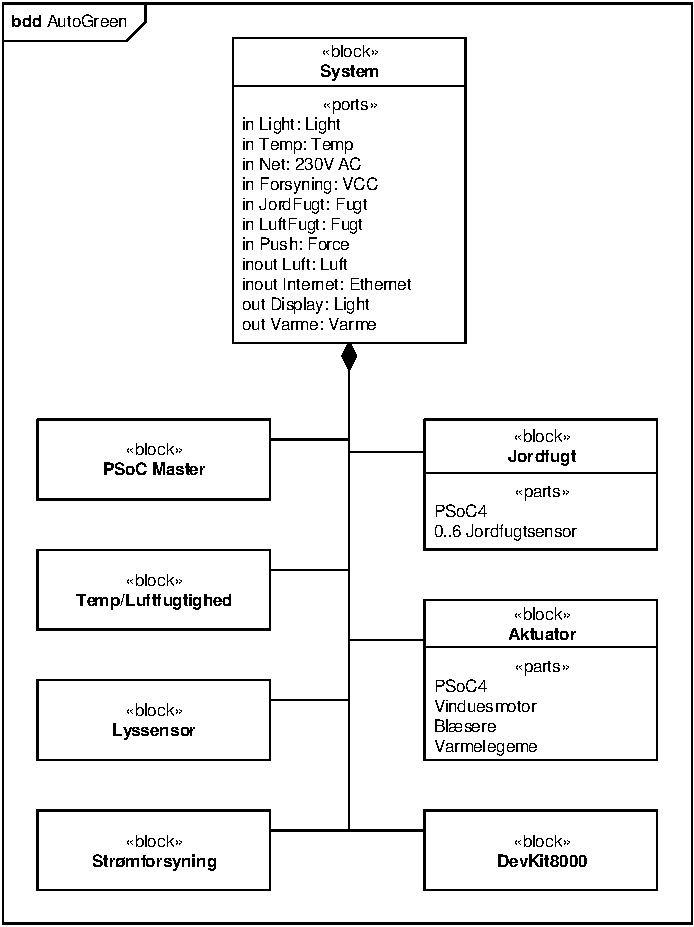
\includegraphics[width={\textwidth-2cm}, trim=0 0 0 0, clip=true] {../fig/bdd_system.pdf}
\caption{BDD for System.}
\label{fig:bdd_system}
\end{figure}

\clearpage

\subsection{IBD'er for System}

\begin{figure}[!h]
\centering 
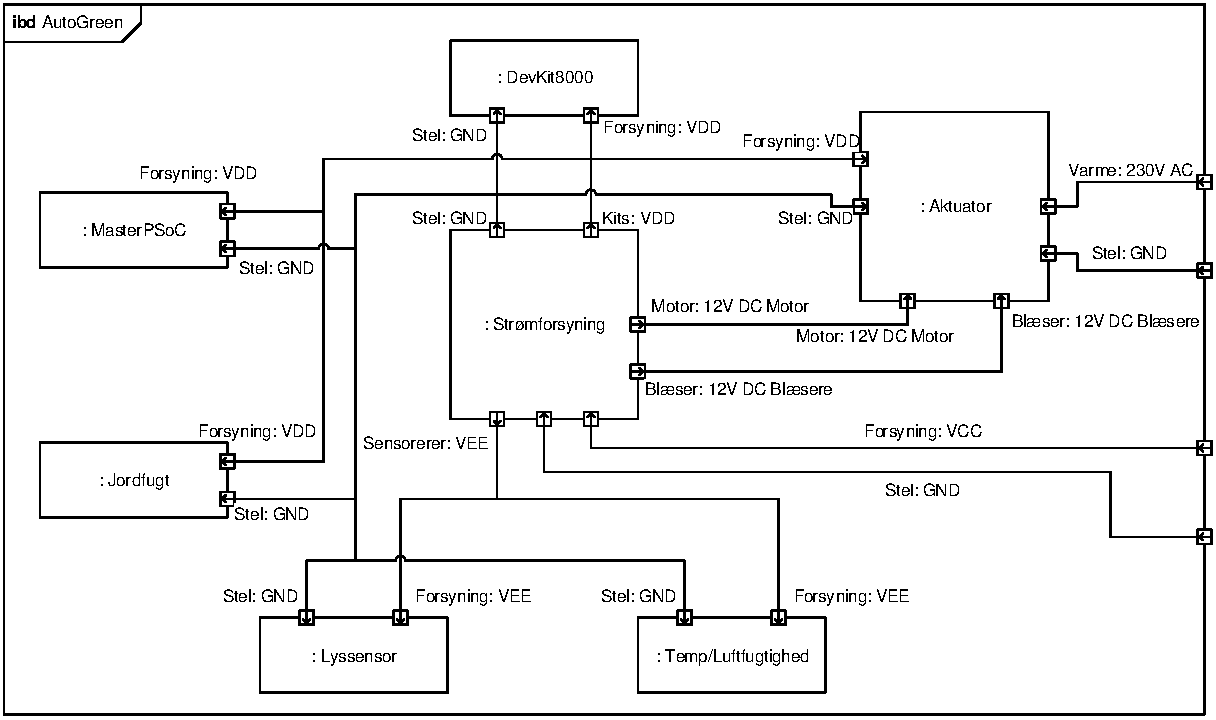
\includegraphics[width={\textheight-65 pt}, angle = 90] {../fig/ibd_system_forsyninger.pdf}
\caption{IBD for forsyninger i systemet.}
\label{fig:ibd_system_forsyn}
\end{figure}

\clearpage

\begin{figure}
\centering 
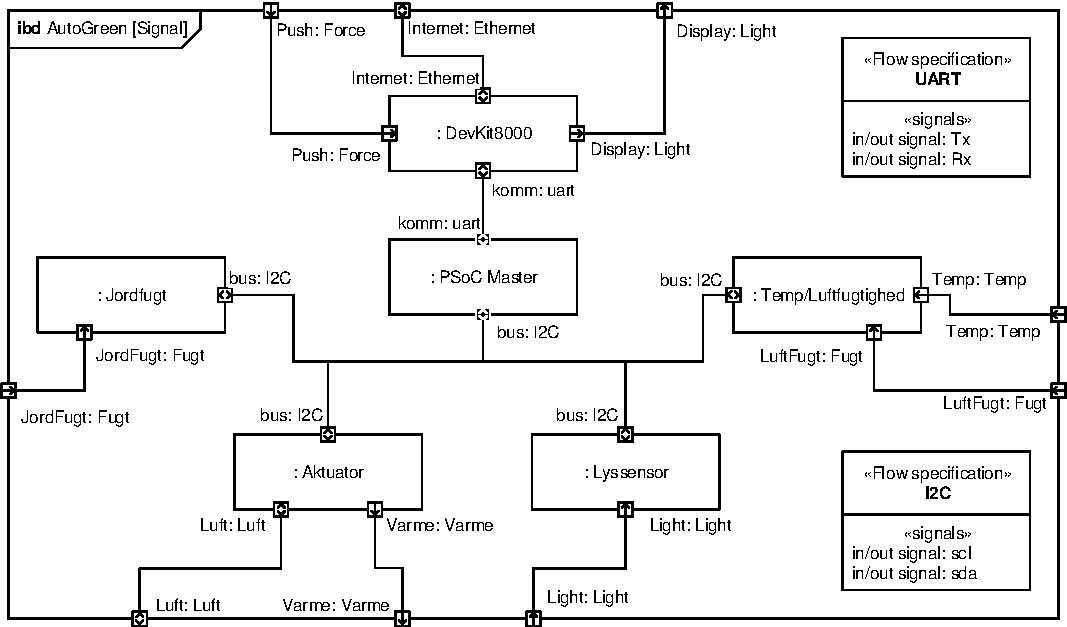
\includegraphics[width={\textheight-25 pt}, angle = 270] {../fig/ibd_system_signaler.pdf}
\caption{IBD for signaler i systemet.}
\label{fig:ibd_system_signal}
\end{figure}

\clearpage

\subsubsection{Strømforsyning}
Forsyner øvrig hardware i systemet, undtagen varmelegemet, Devkit8000 samt sensorer. Blokken forsynes fra en laboratorieforyning.
\subsubsection{DevKit8000}
Systemets brugerflade, er samtidigt controller for systemet. 
\subsubsection{PSoC Master}
PSoC4 Pioneer Kit, der har til opgave at kommunikere via UART med DevKit8000 og via \IIC med slaver.  
\subsubsection{Temp/Luftfugtighed}
Denne blok indeholder en sensor med \IIC interface og måler temperatur og luftfugtighed i det fysiske drivhus.
\subsubsection{Lyssensor}
Består af en sensor med \IIC interface og måler lysintensitet i det fysiske drivhus. 
\subsubsection{Jordfugt}
Denne blok indeholder op til seks analoge jordfugtsensorer, som vha. et PSoC4 Pioneer Kit er koblet på systemets \IIC bus.
\subsubsection{Aktuator}
Denne blok indeholder et PSoC4 Pioneer Kit, der fungerer som \IIC slave og styrer systemets aktuatorer. 

\clearpage

\subsection{IBD for Aktuator}

\begin{figure}[h]
\centering 
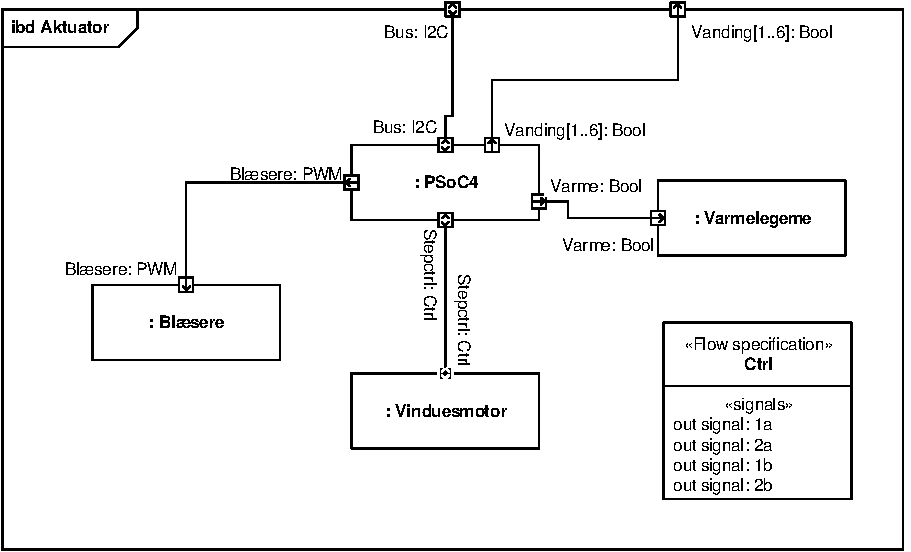
\includegraphics[width={\textwidth}, trim=0 0 0 0, clip=true] {../fig/ibd_aktuator.pdf}
\caption{IBD for Aktuator}
\label{fig:ibd_aktuator}
\end{figure}

\subsubsection{PSoC4}
PSoC blokken består af et PSoC4 Pioneer Kit, der agerer slave på \IIC bussen. 
\subsubsection{Vinduesmotor}
Denne blok består af en steppermotor, der styrer vinduet i det fysiske drivhus.
\subsubsection{Varmelegeme}
Varmelegeme med formål at hæve temperaturen i det fysiske drivhus. Varmelegemet styres af PSoC4 blokken, og det forsynes direkte fra elnettet (230V AC). 
\subsubsection{Blæsere}
Denne blok består af fire blæsere, som kan ventilere luften i det fysiske drivhus. Blæserne styres af PSoC4, og de forsynes fra Strømforsyning. 

\clearpage

\subsection{IBD for Jordfugt}

\begin{figure}[h]
\centering 
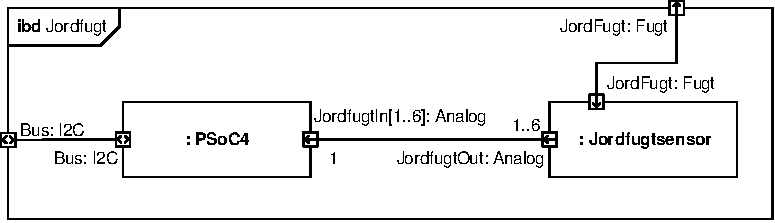
\includegraphics[width={\textwidth}] {../fig/ibd_jordfugt.pdf}
\caption{IBD for Jordfugt}
\label{fig:ibd_jordfugt}
\end{figure}

\subsubsection{PSoC4}
PSoC4 Pioneer Kit, der agerer slave på \IIC-bussen. 
\subsubsection{Jordfugtsensor}
Denne blok indeholder en analog sensor, der måler jordfugt ved en plante i det fysiske drivhus. Der kan kobles op til seks af disse til PSoC4.

\clearpage

\subsection{Signalbeskrivelser}
\label{subsec:signalbeskrivelser}

%\LTXtable{\textwidth}{Systemarkitektur/HWarkitektur/signalbeskrivelser.tex}

\begin{table}[h]
\begin{tabularx}{\textwidth}{| l | >{\raggedright}X | >{\raggedright}X | >{\raggedright\arraybackslash}X |>{\raggedright}X |}
\hline
	\textbf{Signaltype} & \textbf{Funktion} & \textbf{Tolerancer} & \textbf{Kommentar}\\ \hline
	VCC & Forsyning til strømforsyning & 12V $\pm$ 0,25V \newline 3A max. & Lab.forsyning  \\\hline	
	VDD & Forsyning til alle PSoC4 Pioneer Kits. & 5V DC $\pm$ 0.15V, \newline 0.5A max & - \\\hline
	VEE & Forsyning til sensorer & 3.3V DC $\pm$ 0.1V, \newline 0.1A max & - \\\hline
	12V DC Blæsere & Forsyning til blæsere. & 12V DC $\pm$ 0,25V, \newline 140mA max. & - \\\hline	
	12V DC Motor & Forsyning til vinduesmotor. & 12V $\pm$ 0,25V, \newline 500mA max. & - \\\hline
	230V AC & Forsyning til varmelegeme og DevKit8000. & 230V AC $\pm$ 10\%, \newline 50 Hz, \newline 0.3A max & - \\\hline
	Analog & Analogt målesignal fra jordfugtmåler. & 0-3.3V $\pm$ 0.1V & - \\\hline	
	Bool & Digitalt signal til styring af vanding og varmelegeme. & 0-3.3V & 1=True: 2.8-3.3V \newline 0=False: 0-0.4V \\\hline	
	Ctrl & Styring af stepper motor & 0-3.3V & 1=True: 2.8-3.3V \newline 0=False: 0-0.4V  \newline Består af fire signaler: \newline 1a, 2a, 1b, 2b \\\hline	
	GND & Stel & 0V & Reference \\\hline	
	I2C & Kommunikation mellem \IIC enheder. & 0-3.3V & 1=True: 2.8-3.3V \newline 0=False: 0-0.4V \newline Består af to signaler: \newline sca og scl \\\hline	
	UART & Kommunikation mellem DevKit8000 og Master & 0-5V & 1=True: 4.5-5V \newline 0=False: 0-0.4V \newline Består af 2 signaler: \newline Tx og Rx \\\hline	
	PWM & Styring af blæsere vha. pulsbreddemodulation. & 0-3.3V \newline 1 kHz & Duty cycle styres fra 0-100\% i trin fra 0-255. 0 svarer til 0\% og 255 svarer til 100\% \\\hline
\end{tabularx}
\caption{Beskrivelse af signaler.}
\label{tbl:signalbeskriv}
\end{table}

\clearpage